% SPDX-FileCopyrightText: 2026 Shayan Abrar
% SPDX-License-Identifier: MIT
% Independent revision, 2026-10-19. Source reviewed: 67440c664f658ccd589f7198ee2182d5820ca7c1.
% Follow-up on the original machine, 2026-10-19/20: test counts, benchmark table and study-artifact export
% updated from reports/jmlr/original-machine-2026-10-19/ and benchmarks/standard-2026-10-19T180346+0000/.
% Author details and disclosures remain to be supplied. See EVIDENCE.md and BUILD.md.
\documentclass[twoside,11pt]{article}
\usepackage{jmlr2e}
\usepackage{lastpage}
\usepackage{booktabs}
\newcommand{\TODO}[1]{\textbf{[#1]}}
\newcommand{\lunarlab}{\textsc{LunarLab}}
\jmlrheading{0}{2026}{1-\pageref{LastPage}}{pending}{}{00-0000}{Shayan Abrar}
\ShortHeadings{LunarLab: Auditable Reward-Design Experiments}{Abrar}
\firstpageno{1}
\begin{document}
\title{LunarLab: Auditable Reward-Design Experiments in Reinforcement Learning}
\author{\name Shayan Abrar \email \TODO{author email required} \\
\addr \TODO{affiliation and complete postal address required}}
\editor{Not assigned}
\maketitle

\begin{abstract}
Reward-design experiments need evidence that optimized reward reflects task performance. \lunarlab{} is an
MIT-licensed toolkit integrating reward accounting, policy evaluation and provenance. Built on Stable-Baselines3
and Gymnasium's LunarLander-v3, it decomposes rewards at each transition, stores episode totals, selects
checkpoints on validation seeds, and tests protected, digest-checked copies on separate seeds. Configuration
hashes and software records connect results to their artifacts. A CLI, Python API and local web application
expose the workflow; optional traces support inspection and re-scoring. Five PPO training seeds per design
illustrate its use: a flawed hover bonus yields high shaped returns but no strict landings in 500 test episodes.
Three distributed policies also expose a portability limit: Windows evaluations match selected summary fields,
whereas Linux trajectories diverge despite similar aggregates. The main workflow is LunarLander-specific;
a separate audit API is demonstrated on CartPole. The contribution is an inspectable experimental process,
not a new learning algorithm. Code: \url{https://github.com/SHAYAN-ABRAR/lunarlab}.
\end{abstract}
\begin{keywords}
reinforcement learning, reward shaping, reward hacking, reproducibility, open-source software
\end{keywords}

\section{Introduction}
A policy can improve its training reward while failing the intended task. Reward gaming concerns this
relationship between objectives \citep{skalse2022gaming}. Auditing reward design requires separate accounts of
original reward, modified reward, and behavioral outcomes, together with evidence identifying the selected
checkpoint and the observations used for selection. These requirements complement established concerns about
RL evaluation and reproducibility \citep{henderson2018matters,agarwal2021precipice}.

\lunarlab{} integrates reward accounting, validation-based selection, protected final-test artifacts, and
diagnostic replay. Researchers can inspect whether a reward modification improves task outcomes, which reward
components explain a trajectory, and whether re-evaluating the same policy preserves an observed failure.
The contribution is this auditable process, rather than a new algorithm.

\section{Workflow and Implementation}
\paragraph{Accounting and diagnostics.} The main pipeline uses Gymnasium's LunarLander-v3
\citep{towers2024gymnasium} and Stable-Baselines3 implementations of PPO and DQN \citep{raffin2021sb3}.
A wrapper computes
\[
 r_{\mathrm{train}}(s,a,s')=w\,r_{\mathrm{orig}}(s,a,s')+\sum_k F_k(s,a,s').
\]
A validated configuration specifies the terms and has a content hash. Shared pure functions compute the
terms for training, evaluation, and trajectory re-scoring. Normal training persists episode totals for
original reward, training reward, and individual terms; per-transition traces are optional. The wrapper
preserves observations and termination signals. Behavioral diagnostics include a hover detector independent
of the chosen reward preset and a strict pad-landing classifier using position, attitude, contact, and
termination information. These task-specific diagnostics are not universal definitions of reward exploitation.

Built-in designs include a time penalty, a deliberately exploitable hover bonus, and potential-based shaping
$F=\alpha(\gamma\Phi(s')-\Phi(s))$. The latter matches the learner's discount, uses zero terminal potential, and distinguishes time-limit
truncation. Property tests check telescoping. The policy-invariance theorem \citep{ng1999shaping} does not
guarantee better finite-budget learning.

\paragraph{Selection and provenance.} Validation and final-test seed lists are checked for duplicates and
overlap. Validation original return selects the checkpoint; final evaluation reports the original return
alongside behavioral outcomes and re-scored training return. At first final testing, the selected checkpoint
is copied to a protected artifact and verified by SHA-256. Interrupted tests reuse that copy. A test-exposure registry marks derived experiments as exploratory but cannot prevent investigator reuse of
test insights. Records include configuration/protocol hashes, transition budgets, software versions, and source revisions.

Checkpoint continuation restores networks, optimizer state, and counters; DQN additionally restores replay
contents and continuation metadata. The simulator and all random-number streams are not restored, so this is
stateful continuation rather than bit-identical uninterrupted training. File integrity, numerical agreement,
and preservation of scientific conclusions are separate questions.

\paragraph{Interfaces and extension.} A CLI, Python API, and React/FastAPI application share the local research core. Replay, re-scoring, robustness,
tuning, and preference workflows require no hosted account. Three-dimensional replay visualizes two-dimensional
simulation. A separate
\texttt{lunarlab.audit} API accepts reward terms and task adapters, with LunarLander consistency tests and a
CartPole example. The main training, checkpoint, and web workflows remain LunarLander-specific.

\section{Relation to Existing Software and Engineering Evidence}
Stable-Baselines3 supplies monitoring, checkpoint tools and separate evaluation environments.
RL Baselines3 Zoo adds recipes, tuning and plotting \citep{raffin2020zoo}. CleanRL emphasizes inspectable
single-file algorithm implementations \citep{huang2022cleanrl}. The \texttt{imitation} library preserves original
rewards alongside learned rewards and implements preference learning \citep{gleave2022imitation}; rliable
provides robust aggregate statistics \citep{agarwal2021precipice}. AI Safety Gridworlds separates reward from
performance measures \citep{leike2017gridworlds}. These are established ideas. \lunarlab{} connects named reward terms, checkpoint identity, held-out evaluation
and diagnostics in one task-specific workflow, with less environmental breadth than general RL libraries.

\paragraph{Testing and packaging.} On Windows~11 the revised source passes all 489 Python tests (86\%
statement and branch coverage) and 15 browser tests; a fresh source-archive installation passes its 189 release
tests. Public CI at base revision \texttt{67440c6} also passed on Linux and Windows. Tests cover reward
identities, seed validation, freezing, continuation and interruption. Tutorial/API and developer documentation
and deterministic archives support use and extension; tests do not establish adoption.

\paragraph{Runtime and memory.} Table~\ref{tab:overhead} reports a benchmark of the revised source.
Hyperparameters and transition counts match across configurations. Relative loop time was
1.021 for accounting and 1.053 for the full training workflow; including its validation and checkpoint work
increased elapsed time to 1.221. These are measurements from three repetitions on one machine, not upper bounds.
The loop interval includes initialization but excludes timed validation and checkpoint operations.
\begin{table}[t]
\centering\small
\begin{tabular}{@{}lrrrr@{}}
\toprule
Configuration & Transitions/s & Loop ratio & Wall ratio & Peak MB \\
\midrule
SB3 + \texttt{Monitor} & $2{,}158\pm22$ & 1.000 & 1.000 & 310 \\
+ reward accounting & $2{,}115\pm29$ & 1.021 & 1.021 & 310 \\
Full training workflow & $2{,}051\pm55$ & 1.053 & 1.221 & 314 \\
\bottomrule
\end{tabular}
\caption{PPO benchmark: 102,400 transitions per run, three repetitions, Windows 11, Intel i7-13620H, one PyTorch
thread. Throughput is mean $\pm$ sample SD; time ratios use mean durations. The full workflow includes 18,780
validation transitions (7.9\,s on average). Peak MB ($10^6$ bytes) is the process peak through training and
checkpointing, sampled before optional replay generation.}
\label{tab:overhead}
\end{table}

\section{Example Audit and Reproducibility Limits}
The primary demonstration trains PPO \citep{schulman2017ppo} with five seeds for each of four reward designs,
using 1,003,520 transitions per run. Checkpoints are selected on ten validation seeds and evaluated on 100
disjoint test seeds per policy. Figure~\ref{fig:study} uses the committed per-policy summaries. The original
reward baseline has an interquartile-mean (IQM) original return of 268.6 and a 97.6\% strict landing rate.
The hover-bonus group has IQM $-33.1$, no strict landings in 500 episodes, and 80\% timeouts. Its mean re-scored
training return is 496.3 while its mean original return is $-23.5$. The discrepancy demonstrates exploitation
of this reward design under the studied configuration; it is not a general detector-validation benchmark.

\begin{figure}[t]
\centering
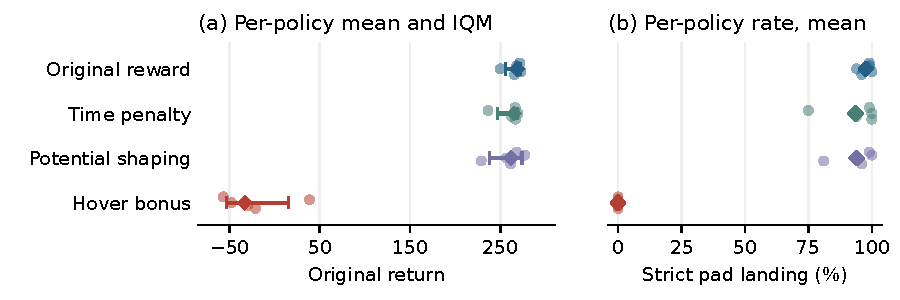
\includegraphics{figures/final_test_audit.pdf}
\caption{Final-test audit for four PPO reward designs. Dots show five policies (100 episodes each); diamonds show return IQM and mean landing rate. Bars: 95\%
percentile intervals from 5,000 training-run bootstrap resamples. Five seeds limit uncertainty resolution;
zero observed landings does not imply zero population success probability.}
\label{fig:study}
\end{figure}

Time-penalty and potential-based shaping obtain IQMs 265.3 and 262.3. Both intervals for probability of
improvement include 0.5; improvement is not established. The bootstrap conditions on fixed evaluation seeds. The broader study has 38 policies and 3,800 final-test
episodes. The repository includes three replayable packages; packages for all 38 were exported without
retraining, and recomputing every summary from their episodes reproduces the published values. Unequal DQN budgets preclude algorithm-superiority claims. Simulated preferences and validation use original
reward; no human study or reward-free learning is claimed.

\paragraph{Re-evaluation evidence.} The three packages contain a PPO baseline, PPO hover-bonus policy, and
DQN baseline. In Windows CI and on the recording machine, all 300 episodes match the five compared summary fields exactly: length, original
return, training return, environment outcome, and strict landing indicator. This does not establish trajectory identity. On Linux, no summaries match exactly; mean returns differ by at most
1.52 and strict landing rates remain 96\%, 0\%, and 29\%, respectively. Individual original returns differ by
up to 0.28, 11.9, and 192. Paired tests detect no aggregate differences after Holm correction, which does not
establish equivalence. Nine open-loop reference traces show early simulator-state differences without greedy-action changes on
recorded observations. This supports simulator-numerics divergence, not a specific compiler cause or portability
of all 38 policies.

\paragraph{Availability and conclusion.}
\lunarlab{} is MIT-licensed; the described version is 0.1.0 \TODO{final source revision and public archive of
the 38-policy bundle}, with source-specific evidence in the repository. Its contribution links reward accounting, selection, and
recorded results. Broader task support and independent research use remain to be demonstrated; numerical
reproduction across platforms and prevention of reward hacking are not guaranteed.
\acks{\TODO{Funding and competing-interest declarations required.}}
\clearpage
\bibliography{references}
\end{document}
